\documentclass[12pt, fullpage,letterpaper]{article}

\usepackage[margin=1in]{geometry}
\usepackage{url}
\usepackage{amsmath}
\usepackage{amssymb}
\usepackage{xspace}
\usepackage{graphicx}
\usepackage{hyperref}
\usepackage{cancel}
%\usepackage{graphicx}
%\usepackage{subfig}
\usepackage{hyperref}
\usepackage{xcolor}
\usepackage{ulem}
\usepackage{cancel}
\usepackage{float}

\def\red{\color{black!30!red}}
\def\blue{\color{blue}}
\def\blackblue{\color{black!40!blue}}


\newcommand{\semester}{Spring 2022}
\newcommand{\assignmentId}{4}
\newcommand{\releaseDate}{31 March, 2022}
\newcommand{\dueDate}{11:59pm, 15 April, 2022}
\newcommand\independent{\protect\mathpalette{\protect\independenT}{\perp}}
\def\independenT#1#2{\mathrel{\rlap{$#1#2$}\mkern2mu{#1#2}}}

\newcommand{\bx}{{\bf x}}
\newcommand{\bw}{{\bf w}}

\title{CS 6190: Probabilistic Machine Learning \semester}
\author{Homework \assignmentId\\ 
{\red Meysam Alishahi (U1323606)}
}
\date{Handed out: \releaseDate\\
  Due: \dueDate}

\begin{document}
\maketitle

% Math commands by Thomas Minka
\newcommand{\var}{{\rm var}}
\newcommand{\Tr}{^{\rm T}}
\newcommand{\vtrans}[2]{{#1}^{(#2)}}
\newcommand{\kron}{\otimes}
\newcommand{\schur}[2]{({#1} | {#2})}
\newcommand{\schurdet}[2]{\left| ({#1} | {#2}) \right|}
\newcommand{\had}{\circ}
\newcommand{\diag}{{\rm diag}}
\newcommand{\invdiag}{\diag^{-1}}
\newcommand{\rank}{{\rm rank}}
% careful: ``null'' is already a latex command
\newcommand{\nullsp}{{\rm null}}
\newcommand{\tr}{{\rm tr}}
\renewcommand{\vec}{{\rm vec}}
\newcommand{\vech}{{\rm vech}}
\renewcommand{\det}[1]{\left| #1 \right|}
\newcommand{\pdet}[1]{\left| #1 \right|_{+}}
\newcommand{\pinv}[1]{#1^{+}}
\newcommand{\erf}{{\rm erf}}
\newcommand{\hypergeom}[2]{{}_{#1}F_{#2}}

% boldface characters
\renewcommand{\a}{{\bf a}}
\renewcommand{\b}{{\bf b}}
\renewcommand{\c}{{\bf c}}
\renewcommand{\d}{{\rm d}}  % for derivatives
\newcommand{\e}{{\bf e}}
\newcommand{\f}{{\bf f}}
\newcommand{\g}{{\bf g}}
\newcommand{\h}{{\bf h}}
%\newcommand{\k}{{\bf k}}
% in Latex2e this must be renewcommand
\renewcommand{\k}{{\bf k}}
\newcommand{\m}{{\bf m}}
\newcommand{\mb}{{\bf m}}
\newcommand{\n}{{\bf n}}
\renewcommand{\o}{{\bf o}}
\newcommand{\p}{{\bf p}}
\newcommand{\q}{{\bf q}}
\renewcommand{\r}{{\bf r}}
\newcommand{\s}{{\bf s}}
\renewcommand{\t}{{\bf t}}
\renewcommand{\u}{{\bf u}}
\renewcommand{\v}{{\bf v}}
\newcommand{\w}{{\bf w}}
\newcommand{\x}{{\bf x}}
\newcommand{\y}{{\bf y}}
\newcommand{\z}{{\bf z}}
%s\newcommand{\l}{\boldsymbol{l}}
\newcommand{\A}{{\bf A}}
\newcommand{\B}{{\bf B}}
\newcommand{\C}{{\bf C}}
\newcommand{\D}{{\bf D}}
\newcommand{\E}{{\bf E}}
\newcommand{\F}{{\bf F}}
\newcommand{\G}{{\bf G}}
\renewcommand{\H}{{\bf H}}
\newcommand{\I}{{\bf I}}
\newcommand{\J}{{\bf J}}
\newcommand{\K}{{\bf K}}
\renewcommand{\L}{{\bf L}}
\newcommand{\M}{{\bf M}}
\newcommand{\N}{\mathcal{N}}  % for normal density
\newcommand{\Dcal}{\mathcal{D}}  % for normal density

%\newcommand{\N}{{\bf N}}
\renewcommand{\O}{{\bf O}}
\renewcommand{\P}{{\bf P}}
\newcommand{\Q}{{\bf Q}}
\newcommand{\R}{{\bf R}}
\renewcommand{\S}{{\bf S}}
\newcommand{\T}{{\bf T}}
\newcommand{\U}{{\bf U}}
\newcommand{\V}{{\bf V}}
\newcommand{\W}{{\bf W}}
\newcommand{\X}{{\bf X}}
\newcommand{\Y}{{\bf Y}}
\newcommand{\Z}{{\bf Z}}

% this is for latex 2.09
% unfortunately, the result is slanted - use Latex2e instead
%\newcommand{\bfLambda}{\mbox{\boldmath$\Lambda$}}
% this is for Latex2e
\newcommand{\bfLambda}{\boldsymbol{\Lambda}}

% Yuan Qi's boldsymbol
\newcommand{\bsigma}{\boldsymbol{\sigma}}
\newcommand{\balpha}{\boldsymbol{\alpha}}
\newcommand{\bpsi}{\boldsymbol{\psi}}
\newcommand{\bphi}{\boldsymbol{\phi}}
\newcommand{\boldeta}{\boldsymbol{\eta}}
\newcommand{\Beta}{\boldsymbol{\eta}}
\newcommand{\btau}{\boldsymbol{\tau}}
\newcommand{\bvarphi}{\boldsymbol{\varphi}}
\newcommand{\bzeta}{\boldsymbol{\zeta}}

\newcommand{\blambda}{\boldsymbol{\lambda}}
\newcommand{\bLambda}{\mathbf{\Lambda}}
\newcommand{\bOmega}{\mathbf{\Omega}}
\newcommand{\bomega}{\mathbf{\omega}}
\newcommand{\bPi}{\mathbf{\Pi}}

\newcommand{\btheta}{\boldsymbol{\theta}}
\newcommand{\bpi}{\boldsymbol{\pi}}
\newcommand{\bxi}{\boldsymbol{\xi}}
\newcommand{\bSigma}{\boldsymbol{\Sigma}}

\newcommand{\bgamma}{\boldsymbol{\gamma}}
\newcommand{\bGamma}{\mathbf{\Gamma}}

\newcommand{\bmu}{\boldsymbol{\mu}}
\newcommand{\1}{{\bf 1}}
\newcommand{\0}{{\bf 0}}

% \newcommand{\comment}[1]{}

\newcommand{\bs}{\backslash}
\newcommand{\ben}{\begin{enumerate}}
\newcommand{\een}{\end{enumerate}}

 \newcommand{\notS}{{\backslash S}}
 \newcommand{\nots}{{\backslash s}}
 \newcommand{\noti}{{\backslash i}}
 \newcommand{\notj}{{\backslash j}}
 \newcommand{\nott}{\backslash t}
 \newcommand{\notone}{{\backslash 1}}
 \newcommand{\nottp}{\backslash t+1}
% \newcommand{\notz}{\backslash z}

\newcommand{\notk}{{^{\backslash k}}}
%\newcommand{\noti}{{^{\backslash i}}}
\newcommand{\notij}{{^{\backslash i,j}}}
\newcommand{\notg}{{^{\backslash g}}}
\newcommand{\wnoti}{{_{\w}^{\backslash i}}}
\newcommand{\wnotg}{{_{\w}^{\backslash g}}}
\newcommand{\vnotij}{{_{\v}^{\backslash i,j}}}
\newcommand{\vnotg}{{_{\v}^{\backslash g}}}
\newcommand{\half}{\frac{1}{2}}
\newcommand{\msgb}{m_{t \leftarrow t+1}}
\newcommand{\msgf}{m_{t \rightarrow t+1}}
\newcommand{\msgfp}{m_{t-1 \rightarrow t}}

\newcommand{\proj}[1]{{\rm proj}\negmedspace\left[#1\right]}
\newcommand{\argmin}{\operatornamewithlimits{argmin}}
\newcommand{\argmax}{\operatornamewithlimits{argmax}}

\newcommand{\dif}{\mathrm{d}}
\newcommand{\abs}[1]{\lvert#1\rvert}
\newcommand{\norm}[1]{\lVert#1\rVert}

%miscellaneous symbols
\newcommand{\ie}{{{i.e.,}}\xspace}
\newcommand{\eg}{{{\em e.g.,}}\xspace}
\newcommand{\EE}{\mathbb{E}}
\newcommand{\VV}{\mathbb{V}}
\newcommand{\sbr}[1]{\left[#1\right]}
\newcommand{\rbr}[1]{\left(#1\right)}
\newcommand{\cmt}[1]{}



\footnotesize
	\begin{itemize}
		\item You are welcome to talk to other members of the class about
		the homework. I am more concerned that you understand the
		underlying concepts. However, you should write down your own
		solution. Please keep the class collaboration policy in mind.
		
		\item Feel free discuss the homework with the instructor or the TAs.
		
		\item Your written solutions should be brief and clear. You need to
		show your work, not just the final answer, but you do \emph{not}
		need to write it in gory detail. Your assignment should be {\bf no
			more than 10 pages}. Every extra page will cost a point.
		
		\item Handwritten solutions will not be accepted.
		
		\item The homework is due by \textbf{midnight of the due date}. Please submit
		the homework on Canvas.
	\end{itemize}

%GMM
%Bayes logistic regression, VB, Laplace, Laplace Hession, 
%LDA 

\section*{Practice  [100 points + 100 bonus]}	
\label{sec:q1}
\begin{enumerate}
	\item~[20 points] Suppose we have a scalar distribution, 
	\[
	p(z) \propto \exp(-z^2)\sigma(10z + 3).
	\]
	\begin{enumerate}
		\item~[3 points] Although the normalization constant is not analytical, we can use Gauss-Hermite quadrature to calculate an accurate approximation. Please base on the example in ``data/example-code/gmq\_example.py'', calculate the numerical approximation of the normalization constant, and report its value. With the normalization constant, please draw the density curve of $p(z)$, in the range $z \in [-5, 5]$. \\
{\bf \red Answer: }{\blackblue 
Setting degree (number of points) to $300$, the normalization constant is $1.169$.
}
		\item~[5 points] Implement the Laplace approximation of $p(z)$, and report the mean and variance of your Gaussian distribution. Draw the density of your Laplace approximation in the same plot as in (a).  \\
{\bf \red Answer: }{\blackblue 
To use the Laplace approximation, we need to compute the MAP and the second derivative at that point. 
Setting 
$$
h(z) = -\log p(z) =  z^2 - \log \sigma(10z + 3), 
$$
we can compute 
$$
h'(z) = 2z - 10(1-\sigma(10z + 3)) 
$$
and 
$$
h''(z) = 2 + 100\sigma(10z+3)(1-\sigma(10z + 3)).
$$
Using an optimization method such as {\it ``L-BFGS-B''} to minimize $h(z)$ (equivalently maximizing $p(z)$),
we obtain $\mu = z_{max} = 0.09471726$ and thus 
$\sigma^2 = 1/h''(z_{max}) = 0.25917088.$
Therefore, Laplace approximation density is $\N(0.095, 0.259).$
}
		\item~[10 points] Use the local variational inference method and EM-style updates as we discussed in the class (for logistic regression) to implement the variational approximation to $p(z)$. Report the form of your approximate distribution, and draw its density in the same plot as above.\\
{\bf \red Answer: }{\blackblue 
It is proven that 
$$\sigma(z)\geq \sigma(\xi)\exp\left\{\frac{z-\xi}{2}-\lambda(\xi)(z^2-\xi^2))\right\},$$
where 
$$\lambda(\xi)=\frac{1}{2\xi}\left[\sigma(\xi)-\frac{1}{2}\right].$$
We can therefore write 
\begin{align*}
p(z) & =\frac{1}{Z}\exp(-z^2)\sigma(10z + 3)\\
& \geq \frac{1}{Z}\exp(-z^2)\sigma(\xi)\exp\left\{\frac{10z+3-\xi}{2}-\lambda(\xi)((10z+3)^2-\xi^2))\right\}\\
& \propto \N\big(z|0,\frac{1}{\sqrt{2}}\big)h(z,\xi).
\end{align*}
and accordingly, 
\begin{align*}
\log p(z) 
&\geq  \log \left(\N\big(z|0,\frac{1}{\sqrt{2}}\big)h(z,\xi)\right) + \text{Const}\\
& \geq -z^2 + \log \sigma(\xi) + \frac{10z+3-\xi}{2}-\lambda(\xi)\left((10z+3)^2-\xi^2)\right) +\text{Const}\\
& = -(1+100\lambda(\xi))z^2 +(5-60\lambda(\xi))z + \text{Const}(\xi).\\
& = -\frac{1}{2\sigma^2}(z^2 - 2\mu z + ) + \cdots  
\end{align*}
To apply the local variational inference method, we should solve 
$$\max\limits_{q,\xi} \EE_{q(z)}\log \frac{\N\big(z|0,\frac{1}{\sqrt{2}}\big)h(z,\xi)}{q(z)}.$$
To use EM-algorithm, we first maximize it to find $q(z)$ given $\xi$ fixed (E-step) and then 
we consider $q(z)$ fixed and maximized it to find $\xi$ (M-step).

In the E-step, same as Mean-Field (or using complete square method), we obtain 
\begin{align*}
q(z) 
& \propto \exp\left\{\log \left(\N\big(z|0,\frac{1}{\sqrt{2}}\big)h(z,\xi^{\rm old})\right)\right\}\\
& \propto \N(z|\mu_0,\sigma_0),
\end{align*}
where 
\begin{equation}\label{estep}
\mu_0 = \mu_0(\xi^{\rm old}) = \frac{5-60\lambda(\xi^{\rm old})}{2+200\lambda(\xi^{\rm old})}
\quad\quad\quad \text{and}\quad\quad\quad 
\sigma_0= \sigma_0(\xi^{\rm old}) =\frac{1}{ \sqrt{2+200\lambda(\xi^{\rm old})}}.
\end{equation}
Therefore, {\bf E-step update} will be 
\begin{equation}\label{E_step}
q(z) =  \N\left(z|\mu_0(\xi^{\rm old}),\sigma_0(\xi^{\rm old})\right).
\end{equation}

Now, in the M-step, we assume $q(z)$ is given and optimize 
\begin{align*}
\mathcal{Q}(\xi,\xi^{\rm old}) 
& = \displaystyle\EE_{q(z)}\log \frac{\N\big(z|0,\frac{1}{\sqrt{2}}\big)h(z,\xi)}{q(z)}\\
& = \EE_{q(z)}\log h(z,\xi) + {\rm Const}\\
& = \EE_{q(z)}\left[\log \sigma(\xi) - \frac{\xi}{2}-\lambda(\xi)\big((10z+3)^2-\xi^2)\big)\right]+ {\rm Const}\\
& = \log \sigma(\xi) - \frac{\xi}{2} -\lambda(\xi)\left(100\sigma^2_0 +(10\mu_0+3)^2 -\xi^2)\right) + {\rm Const}.
\end{align*}
We now set the derivative with respect to $\xi$ equal to zero which implies 
$$0 = \lambda'(\xi)\left(100\sigma^2_0 +(10\mu_0+3)^2 -\xi^2\right).$$
Therefore, using the same trick as explained in the class ($\lambda'(\xi)\neq 0$ for $\xi>0$),
the {\bf M-step update} will be 
\begin{equation}\label{M_step}
\xi^{\rm new} =\sqrt{100\sigma^2_0 +(10\mu_0+3)^2}.
\end{equation}
Using these updates rules, we obtain the variational approximation  
$$q(z) = \N(z|\mu = 0.307,\sigma = 0.329).$$
}

		\item~[2 points] By comparing the ``ground-truth'' (from (a)) and the approximations (from (b,c)), what do you observe and conclude?\\
{\bf \red Answer: }{\blackblue 
\begin{figure}[h]
\centering
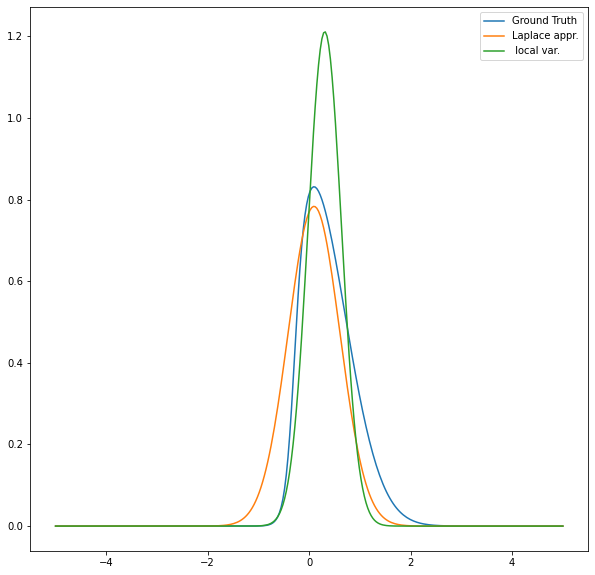
\includegraphics[width=0.5\linewidth]{Images/Q1.png} 
\caption{Ground-truth, Laplace, and local variational approximations} \label{fig:Q1}
\end{figure}
}

	\end{enumerate}

	\item~[50 points] Let us work on a real-world dataset we have met before. Please download the data from the folder``data/bank-note''. The features and labels are listed in the file ``data-desc.txt''. The training data are stored in the file ``train.csv'', consisting of $872$ examples. The test data are stored in ``test.csv'', and comprise of $500$ examples. In both the training and testing datasets, feature values and labels are separated by commas. We assign the feature weight vector $\w$ a standard normal prior $\N(\0, \I)$.  
	\begin{enumerate}
		\item~[7 points] Implement the standard Laplace approximation to the posterior distribution of the feature weight vector. Report your approximate posterior. Now, use Gauss-Hermite quadrature to implement the calculation of the predictive distribution. Please be careful: \textbf{you need to do a proper variable transformation in the integral before applying the Gauss-Hermite quadrature because you integrate  with a Gaussian like $\N(x|\mu, \sigma^2)$ rather than $\exp(-x^2)$!} Now we test the performance with two measures. First, we calculate the inner-product between the posterior mean of the weight vector and the feature vector of each test example, and throw the inner-product into the sigmoid function to calculate the probability that the test example is positive. If the probability is no less than 0.5, we classify the example to be positive (\ie 1) otherwise we classify the example to be negative (\ie 0). Report the prediction accuracy. Second, we calculate the average predictive likelihood of the test samples, namely we evaluate the predictive density value of each test sample based on the predictive distribution and then take an average.  Note that in Bayesian learning, the predictive likelihood includes all the information of the (approximate) posterior distribution, hence is more preferred in the evaluation. \\
{\bf \red Answer: }{\blackblue 
{\red Note that we have added $1$ as the fisrt entry to each feature vector to consider the bias term. }\\
{\bf Standard Laplace approximation to the posterior distribution $p(\w|\t)$} is  
$$q(\w) = \N(\w|\bmu_0,\bSigma_0)$$
where 
$$\bmu_0 = [ 2.85594016, -2.69321758, -1.59105678, -1.8992619 , -0.17689812]^\top$$
and
$$\bSigma_0 = \left[\begin{array}{ccccc}
0.13679752 & -0.05634869 & -0.02708631 & -0.0406641 &  0.02068531\\
-0.05634869 &  0.11964241 &  0.05318788 &  0.07181374 &  0.00963915\\
-0.02708631 &  0.05318788 & 0.05011859 &  0.05299433 &  0.02319023\\
-0.0406641 &  0.07181374 &  0.05299433 &  0.06217003 &  0.0196692\\
0.02068531 &  0.00963915 &  0.02319023 &  0.0196692  &  0.0382288
\end{array}\right].$$
{\bf Performance on the test set using $\bmu_0 = \w_{MAP}$:}\\
{\bf Accuracy: 99\%}

{\bf Calculation of the predictive distribution:}\\
Note that we know $\w|\t \sim \N(\bmu_0,\bSigma_0)$ (approximately). 
For a given feature vector $\x$, setting $a = \x^\top \w$, we obtain 
$$a|\t \sim \N(\x^t\bmu_0, \x^\top\bSigma_0 \x).$$
Therefore, setting $m = \x^t\bmu_0$ and $s^2 = \x^\top\bSigma_0 \x$, 
\begin{align*}
p(t=1|\x) &=  \int \sigma(a)p(a|\t)\d a\\
& \approx \int \sigma(a)\N(a|m, s^2)\d a\\
& =  \frac{1}{\sqrt{\pi}}\int e^{-z^2}\sigma(\sqrt{2}s z+m)\d z.
\end{align*}
Now, we can apply Gauss-Hermite quadrature to compute this integral. 

\bigskip

{\bf Performance on the test set using predictive distribution:}\\
{\bf Accuracy: 99\%\\
Average Predictive Likelihood: 0.974324189967849}



}
		\item~[3 points] Implement Laplace approximation with the diagonal Hessian. Report the approximate posterior distribution of the feature weights, the prediction accuracy and average predictive likelihood. \\
{\bf \red Answer: }{\blackblue 
It means that we assume $q(\w) = \prod\limits_{i=1}^d q(w_i)$.
In this case, for each $i\in[d]$, we want to approximate  
$$\log q(w_i)\approx  \log q(\mu_i) - \frac{1}{2}\sigma_i^{-2}(w-\mu_i).$$
Using the same approach as in class was done, we obtain 
that the $\mu_0$ would be the same as previous part and the $\bSigma_0$ is a diagonal matrix whose digonal entries are the same as prevous part, i.e., $$\bmu_0 = [ 2.85594016, -2.69321758, -1.59105678, -1.8992619 , -0.17689812]^\top$$
and
$$\bSigma_0 = \left[\begin{array}{ccccc}
0.13679752 & 0 & 0 & 0 &  0\\
0 &  0.11964241 &  0 &  0 &  0\\
0 &  0 & 0.05011859 &  0 &  0\\
0 &  0 &  0 &  0.06217003 &  0\\
0 &  0 &  0 &  0  &  0.0382288
\end{array}\right].$$


{\bf Performance on the test set using predictive distribution:}\\
{\bf Accuracy: 99\%\\
Average Predictive Likelihood: 0.9139297763783802}

}
		\item~[20 points] Implement variational logistic regression we introduced in the class. Use EM-style updates. Report the variational posterior of the feature weight vector you obtained (\ie a multivariate Gaussian). Report the prediction accuracy and average predictive likelihood. \\
{\bf \red Answer: }{\blackblue 
We say that the E-updates are:
$$\m_N = S_N\left(S_0^{-1}m_0 + \sum\limits_{n=1}^N(t_n-\frac{1}{2}\right)\phi_n$$
and 
$$\s_N = s_0^{-1}+2\sum\limits_{n=1}^n\lambda(\xi_n) \phi_n\bphi_n^\top.$$
Also, the M-step is:
$$(\xi_n^{\rm new})^2 = \bphi_n^\top\mathbb{E}(S_N+\m_N\m_N^\top)\bphi_n.$$
Implementing these updates, we obtain
$$\bmu = [ 2.89882616, -2.77086021, -1.63751078, -1.95377589, -0.19364377]$$
and 
$$\bSigma_0 = \left[\begin{array}{ccccc}
0.0287931 & -0.00270207 & -0.00196961 & -0.0041901 &  0.00504233\\
-0.00270207 &  0.00360754 & -0.00021745 &  0.00078054 & -0.001883 \\
-0.00196961 & -0.00021745 &  0.00189673 &  0.00157568 &  0.00167853\\
 -0.0041901  &  0.00078054 &  0.00157568 &  0.0022857 &  0.00045613\\
0.00504233  & -0.001883  &  0.00167853 &  0.00045613 &  0.00640488
\end{array}\right].$$
{\bf Accuracy: 0.99\%}\\
{\bf Predictive Likelihood: 0.9770066184539451}




}
		\item~[15 points] Implement variational logistic regression we introduced in the class.  But this time, you will use the fully factorized posterior,   $q(\w)= \prod_i q(w_i)$ where $w_i$ is $i$-th element in the weight vector $\w$. In the E step, please use the standard mean-field update to alternatively optimize each $q(w_i)$ given all the others fixed. Report your variational posterior (\ie diagonal Gaussian), the prediction accuracy and average predictive likelihood on the test data.  \\
{\bf \red Answer: }{\blackblue 
We already know that (see page 499 of the book: Equations 10.149 - 10.151)
\begin{align*}
p(\t, \w) & = p(\w) p(\t|\w) \\
&\geq p(\w) \underbrace{\prod_{n=1}^N\sigma(\xi_n)\exp\left\{\w^\top \bphi_nt_n - (\w^\top\bphi_n + \xi_n)/  2 - \lambda(\xi_n)\left([w^\top\bphi_n]^2-\xi^2_n\right)\right\}}_{=h(\w,\xi)}
\end{align*}
and thus 
\begin{align}
\log p(\t, \w) & = \log p(\w) p(\t|\w)\nonumber \\
&\geq  \log p(\w)h(\w,\bxi)\nonumber\\
&= -\frac{1}{2}\w^\top\w + \sum\limits_{n=1}^N\Big( \log\sigma(\xi_n) + \nonumber \\
&\quad   \w^\top \bphi_n t_n - (\w^\top\bphi_n + \xi_n)/ 2 - \lambda(\xi_n)\left([w^\top\bphi_n]^2-\xi^2_n\right)\Big)\label{mainvar}.
\end{align}
In Variotional approximation, we want to solve 
\begin{equation}\label{eq1}
\max\limits_{q(\w), \bxi}\overbrace{\mathbb{E}_{q(\w)}\log\Big\{\frac{p(\w)h(\w,\bxi)}{q(\w)}}^{{\red \quad\quad= \mathcal{L}(\q,\bxi)}}\Big\}.
\end{equation}
We have the assumption that the posterior is the fully factorized $\q(\w)= \prod_i q(w_i)$. 
Plug this assumption in omptimization~\ref{eq1} and using EM-algorithm, trying to find the posterior $q(w_i)$,  in the E-step, we maximize the above objective function $\mathcal{L}(\q,\bxi)$
 with respect to each $q(w_i)$ in turn assuming that the other factors $q_j(w_j)$ (for $j\neq i$) and $\bxi$ are fixed.
 In this case, 
 
\begin{align}
\mathcal{L}(q_i) & = \int \q(\w)\log\Big\{\frac{p(\w)h(\w,\bxi)}{q(\w)}\Big\}\d\w\nonumber\\
& = \int q(w_i)\Big\{\underbrace{\int\prod_{j\neq i}q(w_j) \log p(\w)h(\w,\bxi)\d\w_{\neg i}}_{
{\red =\mathbb{E}_{\prod_{j\neq i} q(w_j)}\left[\log p(\w)h(\w,\bxi)\right]}}
\Big\}\d w_i - \int q(w_i)\log q(w_i)\d w_i + {\rm Const}.\nonumber\\
& = \int q(w_i)\underbrace{\mathbb{E}_{\prod_{j\neq i} q(w_j)}\left[\log p(\w)h(\w,\bxi)\right]}_{{\red =\log \tilde{g}(w_i,\bxi) + C}}\d w_i - \int q(w_i)\log q(w_i)\d w_i + {\rm Const}\nonumber\\
& = - {\rm KL}\big(q(w_i)\|\tilde{g}(w_i,\bxi)\big) +{\rm Const}.\label{KLD}
\end{align}

Note that, for a fixed $\bxi$,  we defined a new distribution $\tilde{g}(w_i,\bxi)$ so that 
$$\log \tilde{g}(w_i,\bxi) = \mathbb{E}_{\prod_{j\neq i} q(w_j)}\left[\log p(\w)h(\w,\bxi)\right] +{\rm Const.}$$
By Equation~\ref{KLD}, maximizing $\mathcal{L}(q_i)$, we are indeed minimizing Kullback-Leibler divergence ${\rm KL}\big(q(w_i)\|\tilde{g}(w_i,\bxi)\big)$ which is simply done by setting 
$$q(w_i) = \tilde{g}(w_i,\bxi) \propto \exp\left\{\mathbb{E}_{\prod_{j\neq i} q(w_j)}\left[\log p(\w)h(\w,\bxi)\right]\right\}.$$ 
So, we need to compute 
$$\mathbb{E}_{\prod\limits_{j\neq i} q(w_j)}\left[\log p(\w)h(\w,\bxi)\right].$$
Using \ref{mainvar}, we obtain 
\begin{align*}
\mathbb{E}_{\prod\limits_{j\neq i} q(w_j)}\left[\log p(\w)h(\w,\bxi)\right] 
& = -\frac{1}{2}\mathbb{E}\left(\w^\top\w\right) + \sum\limits_{n=1}^N\Big\{ \log\sigma(\xi_n) +  \mathbb{E}\left(\w^\top\right) \bphi_n t_n\\
 &\quad  - \Big(\mathbb{E}\left(\w^\top\right)\bphi_n + \xi_n\Big)/ 2 - \lambda(\xi_n)\left(\mathbb{E}\left([\w^\top\bphi_n]^2\right)-\xi^2_n\right)\Big\}\\
 & = -\frac{1}{2}w_i^2 +\sum_{n=1}^N\left\{ \phi^{(n)}_i(t_n-\frac{1}{2})w_i -\lambda(\xi_n)\Big((w_i\phi^{(n)}_i)^2 +2w_i\phi^{(n)}_i\sum_{j\neq i}\mu_j\phi^{(n)}_j\Big)\right\} +C\\
 & = -\frac{1}{2}\left(1+2\sum_{n=1}^N\lambda(\xi_n)(\phi^{(n)}_i)^2\right)w_i^2 \\
 &\quad +\sum_{n=1}^N\phi^{(n)}_i\left(t_n -\frac{1}{2} - 2\lambda(\xi_n)\sum_{j\neq i}\mu_j\phi^{(n)}_j\right)w_i + C.
\end{align*}
Therefore, in {\bf M-step}, we do the following updates (for $i=1,\ldots,d$),
$$(\sigma_i^{\rm new})^2 = \frac{1}{1+2\sum\limits_{n=1}^N\lambda(\xi_n)(\phi^{(n)}_i)^2}$$
and 
$$\mu_i^{\rm new} = (\sigma_i^{\rm new})^2\sum_{n=1}^N\phi^{(n)}_i \left(t_n-\frac{1}{2} - 2\lambda(\xi_n)\sum_{j\neq i}\mu_j\phi^{(n)}_j\right).$$

In the M-step, we consider $\w$ fixed and then solve Optimization~\ref{eq1} for $\bxi$. 
\begin{align*}
\mathcal{L}(\bxi) & =  \mathbb{E}_{\q(\w)}\log\Big\{\frac{p(\w)h(\w,\bxi)}{\q(\w)}\Big\} \\  
& = -\frac{1}{2}\mathbb{E}[\w]^\top\mathbb{E}[\w] + \sum\limits_{n=1}^N\Big( \log\sigma(\xi_n) +\mathbb{E}[\w]^\top \bphi_n t_n - (\mathbb{E}[\w]^\top\bphi_n + \xi_n)/ 2 - \lambda(\xi_n)\left(\mathbb{E}[\w^\top\bphi_n]^2-\xi^2_n\right)\Big) \\
& = \sum\limits_{n=1}^N\Big( \log\sigma(\xi_n)  - \xi_n/ 2 - \lambda(\xi_n)\left(\mathbb{E}[\w^\top\bphi_n]^2-\xi^2_n\right)\Big) + {\rm Const.}
\end{align*}
Setting the derivative of $\mathcal{L}(\bxi)$ to zero, we obtain the M-step update rule as follows:
\begin{align*}
\xi^2_n & = \mathbb{E}[\w^\top\bphi_n]^2\\
%& =  \mathbb{E}[\bphi_n^\top\w\w^\top\bphi_n]\\
%& =  \bphi_n^\top\mathbb{E}[\w\w^\top]\bphi_n\\
%& = \bphi_n^\top\left({\rm cov}(\w) + \mathbb{E}(\w)\mathbb{E}(\w)^\top\right)\bphi_n\\
& = \var(\w^\top\bphi_n) + \mathbb{E}^2[\w^\top\bphi_n]\\
& = \sum_{i=1}^d\var(\w_i)\left(\bphi_i^{(n)}\right)^2 + \left(\sum_{i=1}^d\mathbb{E}(w_i)\bphi_i^{(n)}\right)^2.
\end{align*}

Using These updates, we get 
$$\bmu = [2.89537268, -2.76699462, -1.63499389, -1.94911109, -0.19317358]$$
and 
$$\bsigma^2 = [0.01532219, 0.00247973, 0.00047451, 0.00058978, 0.00290673].$$
Indeed, for each $i\in[d]$, 
$$q(w_i)\sim \N(\mu_i,\bsigma_i^2).$$

{\bf Accuracy: 99\%}\\
{\bf Predictive Likelihood: 0.9769986161734513}
}   
		 
		\item~[5 points] Compare the results of the above four approximations. What do you observe and conclude?\\
{\bf \red Answer: }{\blackblue 
Although all the above methods perform almost the same based on test (predictive) accuracy, the predictive likelihood for the variational inference surpasses the other methods. This indicates that by using variational approximation methods we get more close to the true posterior distribution. }
	\end{enumerate}

	\item~[30 points] Gaussian Mixture Model (GMM). Please download the data ``data/faithful/faithful.txt''  from Canvas. Each row is a sample, including 2 features. Please normalize the features in each column to be in [-1, 1]. Specifically, denote the column by $\x$; then we compute for each $x_i \leftarrow (x_i - \mathrm{mean}(\x))/(\max(\x) - \min(\x))$. 
	\begin{enumerate}
		\item~[20 points] Implement EM algorithm for GMM. Set the number of clusters to $2$. Initialize the cluster centers to be [-1, 1] and [1,-1], and the covariance matrix to be $0.1\cdot\I$ for both clusters. Run your EM algorithm for $100$ iterations. For iteration $1$, $2$, $5$, $100$, please draw the figures showing the corresponding cluster centers and memberships. Specifically, for each figure, first draw the scatter plots of the data points and your cluster centers. Each data point is assigned to the cluster that has a great posterior probability to include that data point. Please draw the cluster memberships with different colors. \\
{\bf \red Answer: }{\blackblue 
See Figure \ref{fig:Q3a}.
\begin{figure}[h]
\centering
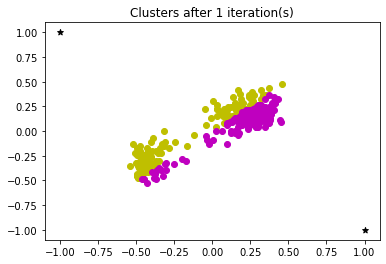
\includegraphics[width=0.4\linewidth]{Images/Q3a1.png} 
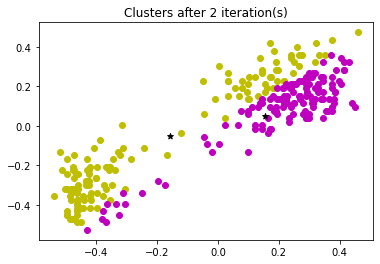
\includegraphics[width=0.4\linewidth]{Images/Q3a2.png} \\
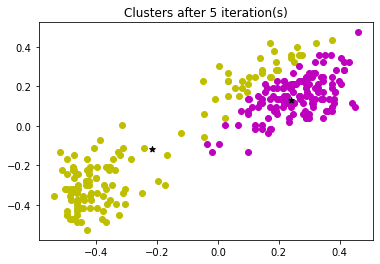
\includegraphics[width=0.4\linewidth]{Images/Q3a3.png} 
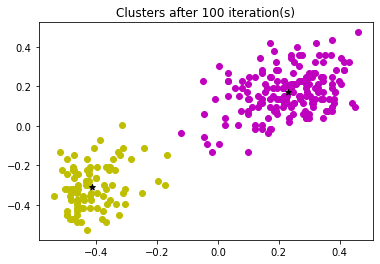
\includegraphics[width=0.4\linewidth]{Images/Q3a4.png} \\
\caption{Clusters with starting the centers to be $(-1, 1)$ and $(1,-1)$} \label{fig:Q3a}
\end{figure}
		
}		
		
\item~[7 points] Now initialize the cluster centers to be [-1, -1] and [1, 1] and covariance matrix to be $0.5 \cdot \I$ for both clusters. Run your EM algorithm for $100$ iterations. Draw the figures showing the cluster centers and memberships for iteration $1$, $2$, $5$, $100$. \\
{\bf \red Answer: }{\blackblue 
See Figure \ref{fig:Q3b}.
\begin{figure}[h]
\centering
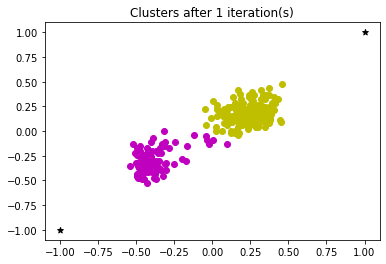
\includegraphics[width=0.4\linewidth]{Images/Q3b1.png} 
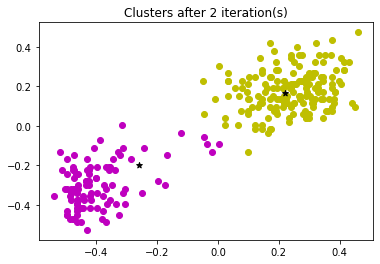
\includegraphics[width=0.4\linewidth]{Images/Q3b2.png} \\
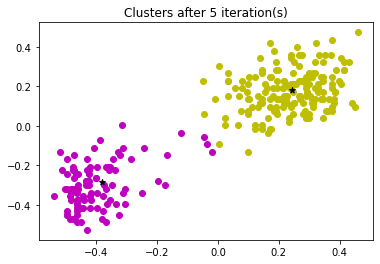
\includegraphics[width=0.4\linewidth]{Images/Q3b3.png} 
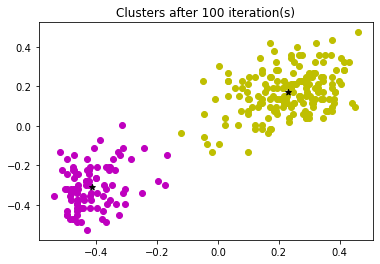
\includegraphics[width=0.4\linewidth]{Images/Q3b4.png} \\
\caption{Clusters with starting the centers to be $(-1, -1)$ and $(1,1)$} \label{fig:Q3b}
\end{figure}
		
}	
\item~[3 points] Compare the results in (a) and (b), what do you observe and conclude?{\bf \red Answer: }{\blackblue 
We can clearly see that the convergence when we initiate the centers as  [-1, -1] and [1, 1] is much faster.  
We can see that the choice [-1, -1] and [1, 1] is more close to the true centers while the points [-1, 1] and [1,-1] are somehow 
symmetric for all the points so they cannot distinguish between clusters truly. 
		}
	\end{enumerate}

	\item~[100 points][\textbf{Bonus}] Latent Dirichlet Allocation (LDA). Please download the pre-processed corpus from ``data/lda''. From ``ap.txt'', you can see the original Associated Press corpus. ``ap.dat'' are the processed data which you will work on. Each row in ``ap.dat'' represents a document. In total, we have $2,246$ documents. The first number in each row is the number of words in the document. The following are a list of  \textbf{word-id}:\textbf{count} items. Word-id starts with 0. The corresponding word list is given in ``vocab.txt''. The first row corresponds to Word-id 0, second, Word-id 1, and continue. 
	
	\begin{enumerate}
		\item~[70 points] Implement the mean-field variational EM algorithm for LDA inference as we discussed in the class. Following the orignal LDA paper ( \url{http://www.cs.columbia.edu/~blei/papers/BleiNgJordan2003.pdf}) to implement the perplexity calculation on test documents (Sec. 7.1). Please randomly select $10\%$ documents as the test set, and run your LDA inference algorithm on the remaining $90\%$ documents. Vary the number of topics from \{5, 10, 15, 20, 50, 100, 200\}. Run your algorithm until convergence or $500$ iterations have achieved. Draw a figure to show how the perplexity vary along with the growth of the topic numbers. What do you observe and conclude?
		\item~[30 points] Set the number of topics to $20$ and run your variational inference algorithm. Examine the top 15 words (\ie with the largest probability) in each learned topic distribution. List a few topics which you think is semantically meaningful and explain why. 
	\end{enumerate}
\end{enumerate}


\end{document}
